\section{Forums}
\subsection{Overview}
Forums are a common feature in learning management systems as it provides a community environment where students can ask questions and discuss content with educators and other students
Many of these built-in forums, however, are very basic and lack sufficient search, sorting and filtering functionality.
In many cases, educators are turning to external, third-party forums in order to take advantage of the more advanced features that they offer.

The aim of this feature is to develop a built-in forum that meets students' and educators' needs so that they no longer need to turn to an external application.

The forum interface consists of the overview page and the individual post pages.

\newpage

\subsubsection{Forum Overview Page}

\begin{figure}[h!]
    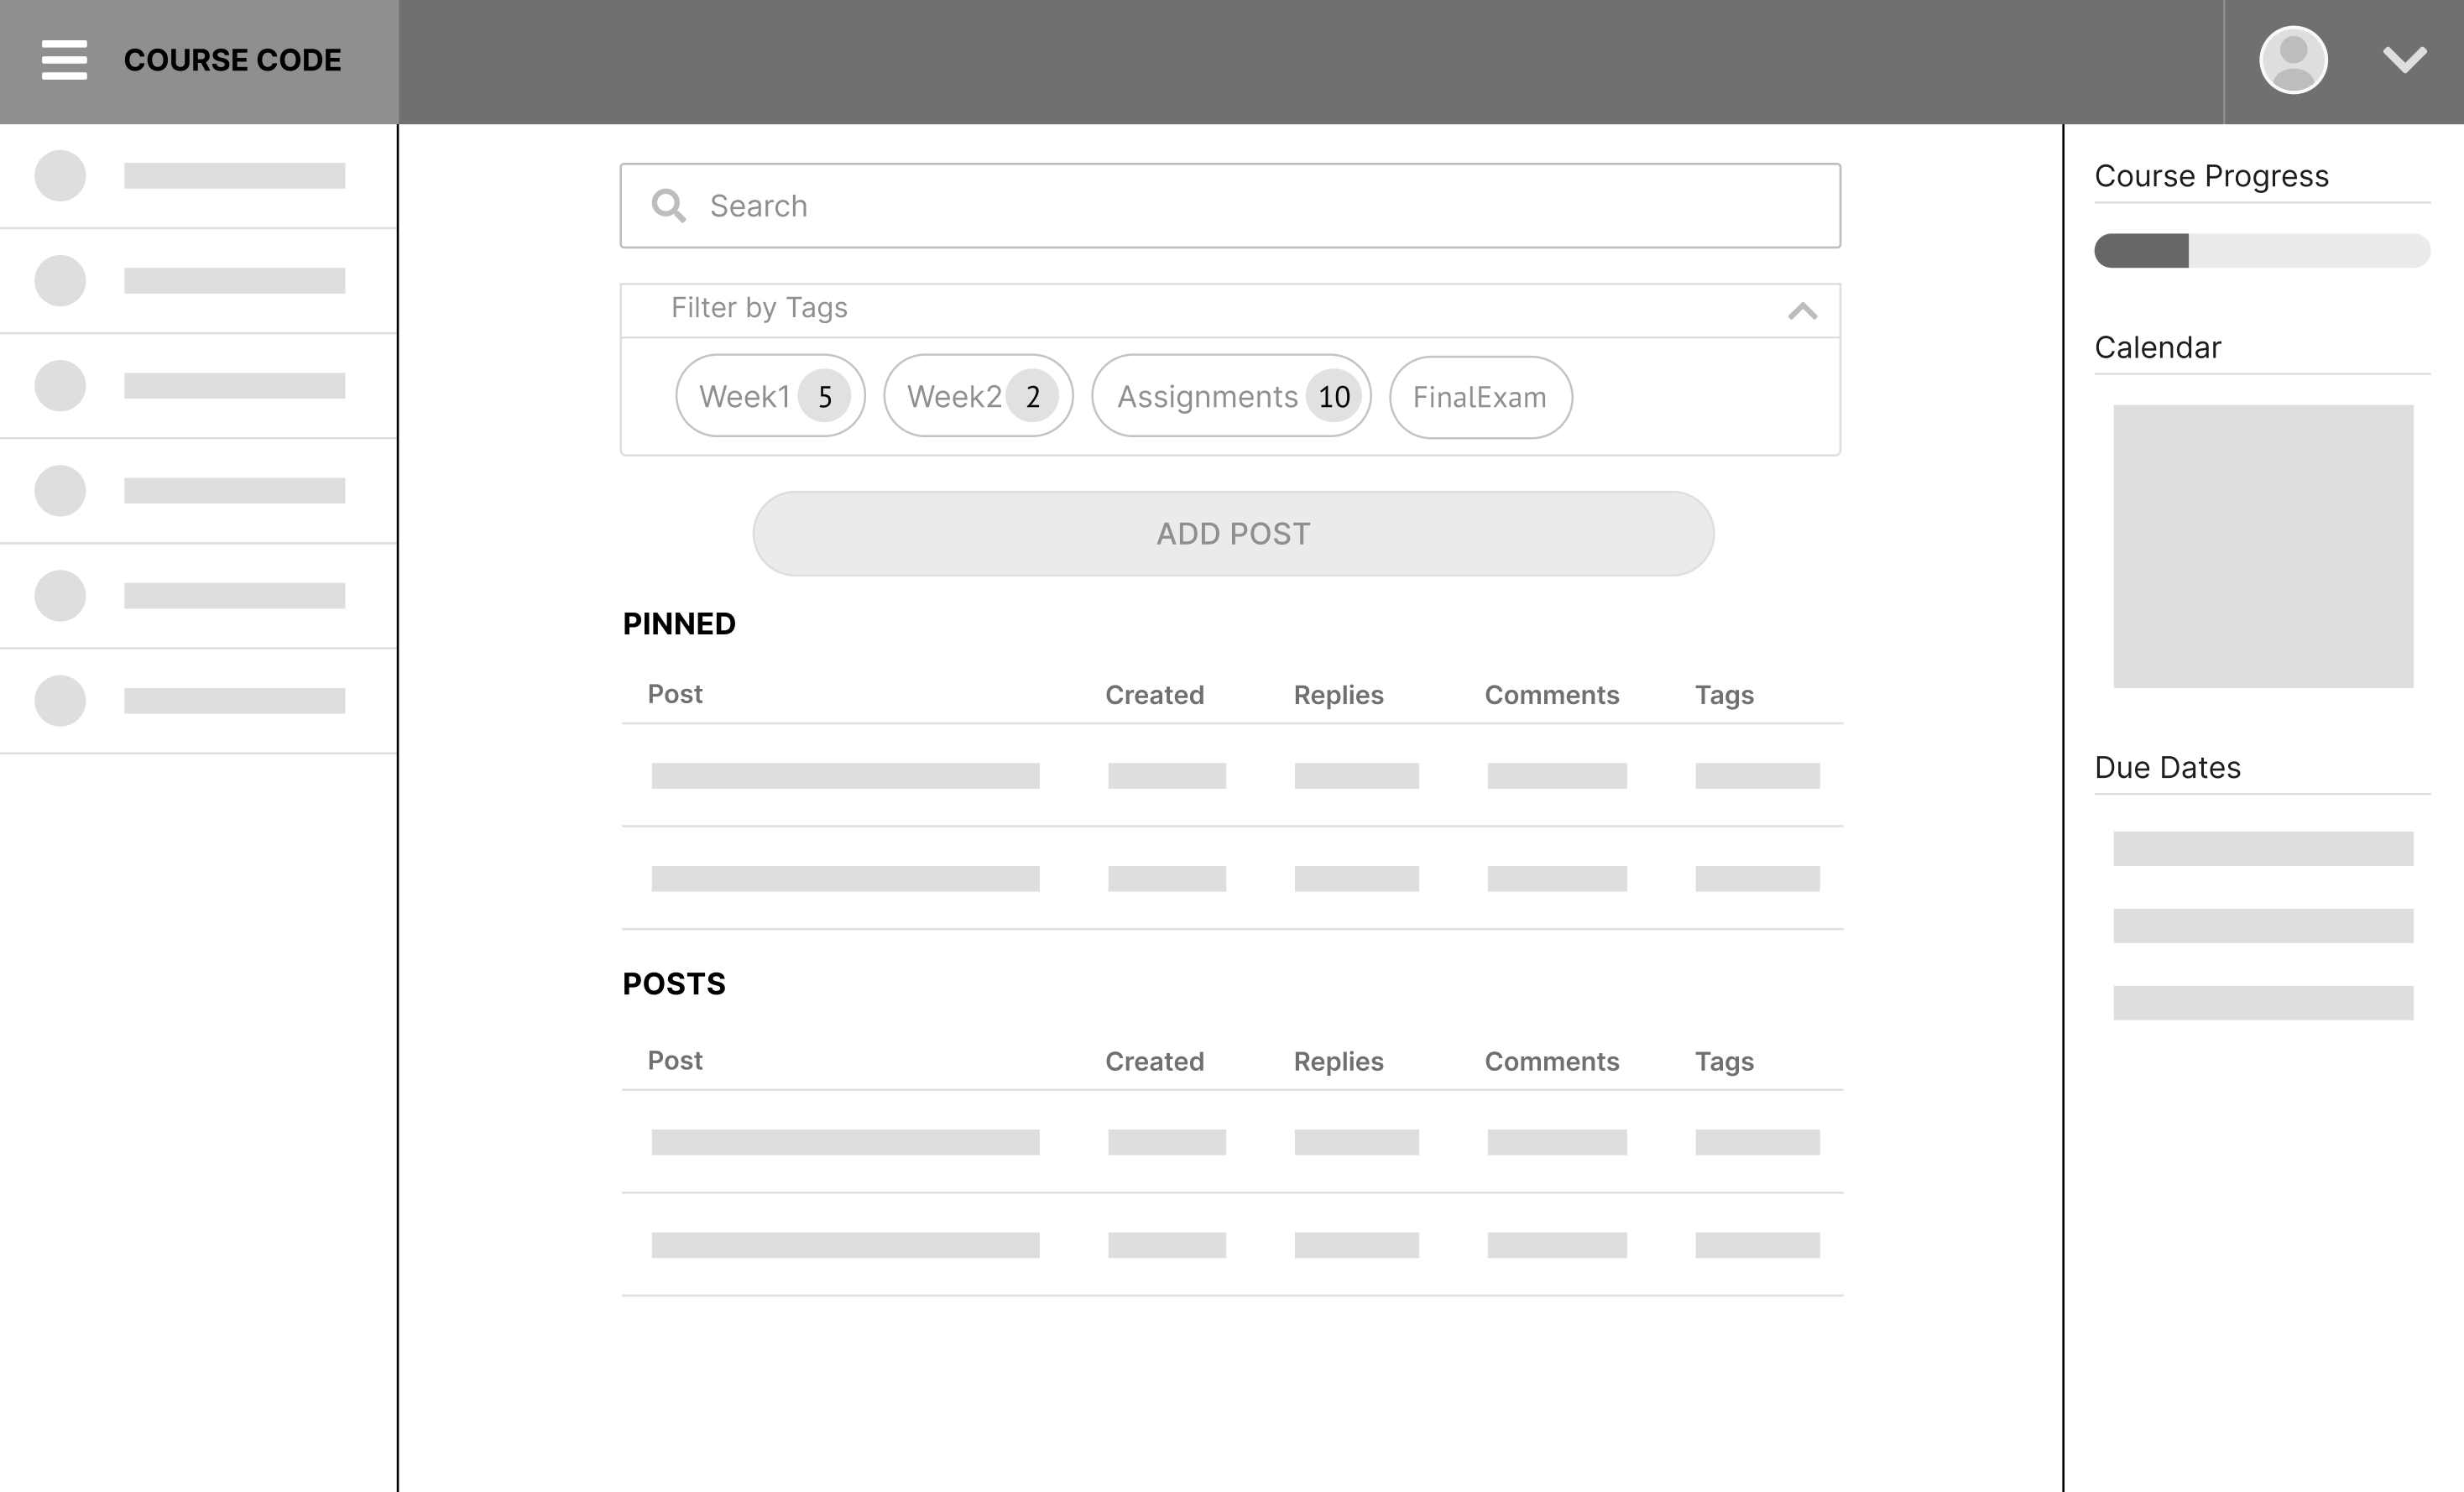
\includegraphics[scale=0.2]{forum-overview-page-student.png}
    \centering
    \caption{Forum overview page for a student}
\end{figure}

In general, the forum overview page consists of a list of posts, as well as search and filtering mechanisms.
The collapsible filter menu allows users to filter the forum post based on pre-defined tags.
Forum posts are ordered such that the list of pinned posts are at the top, followed by the remaining posts in chronological order.
Each row in the table includes the post title, date created, number of replies, number of comments and the associated tags.

\begin{figure}[h!]
    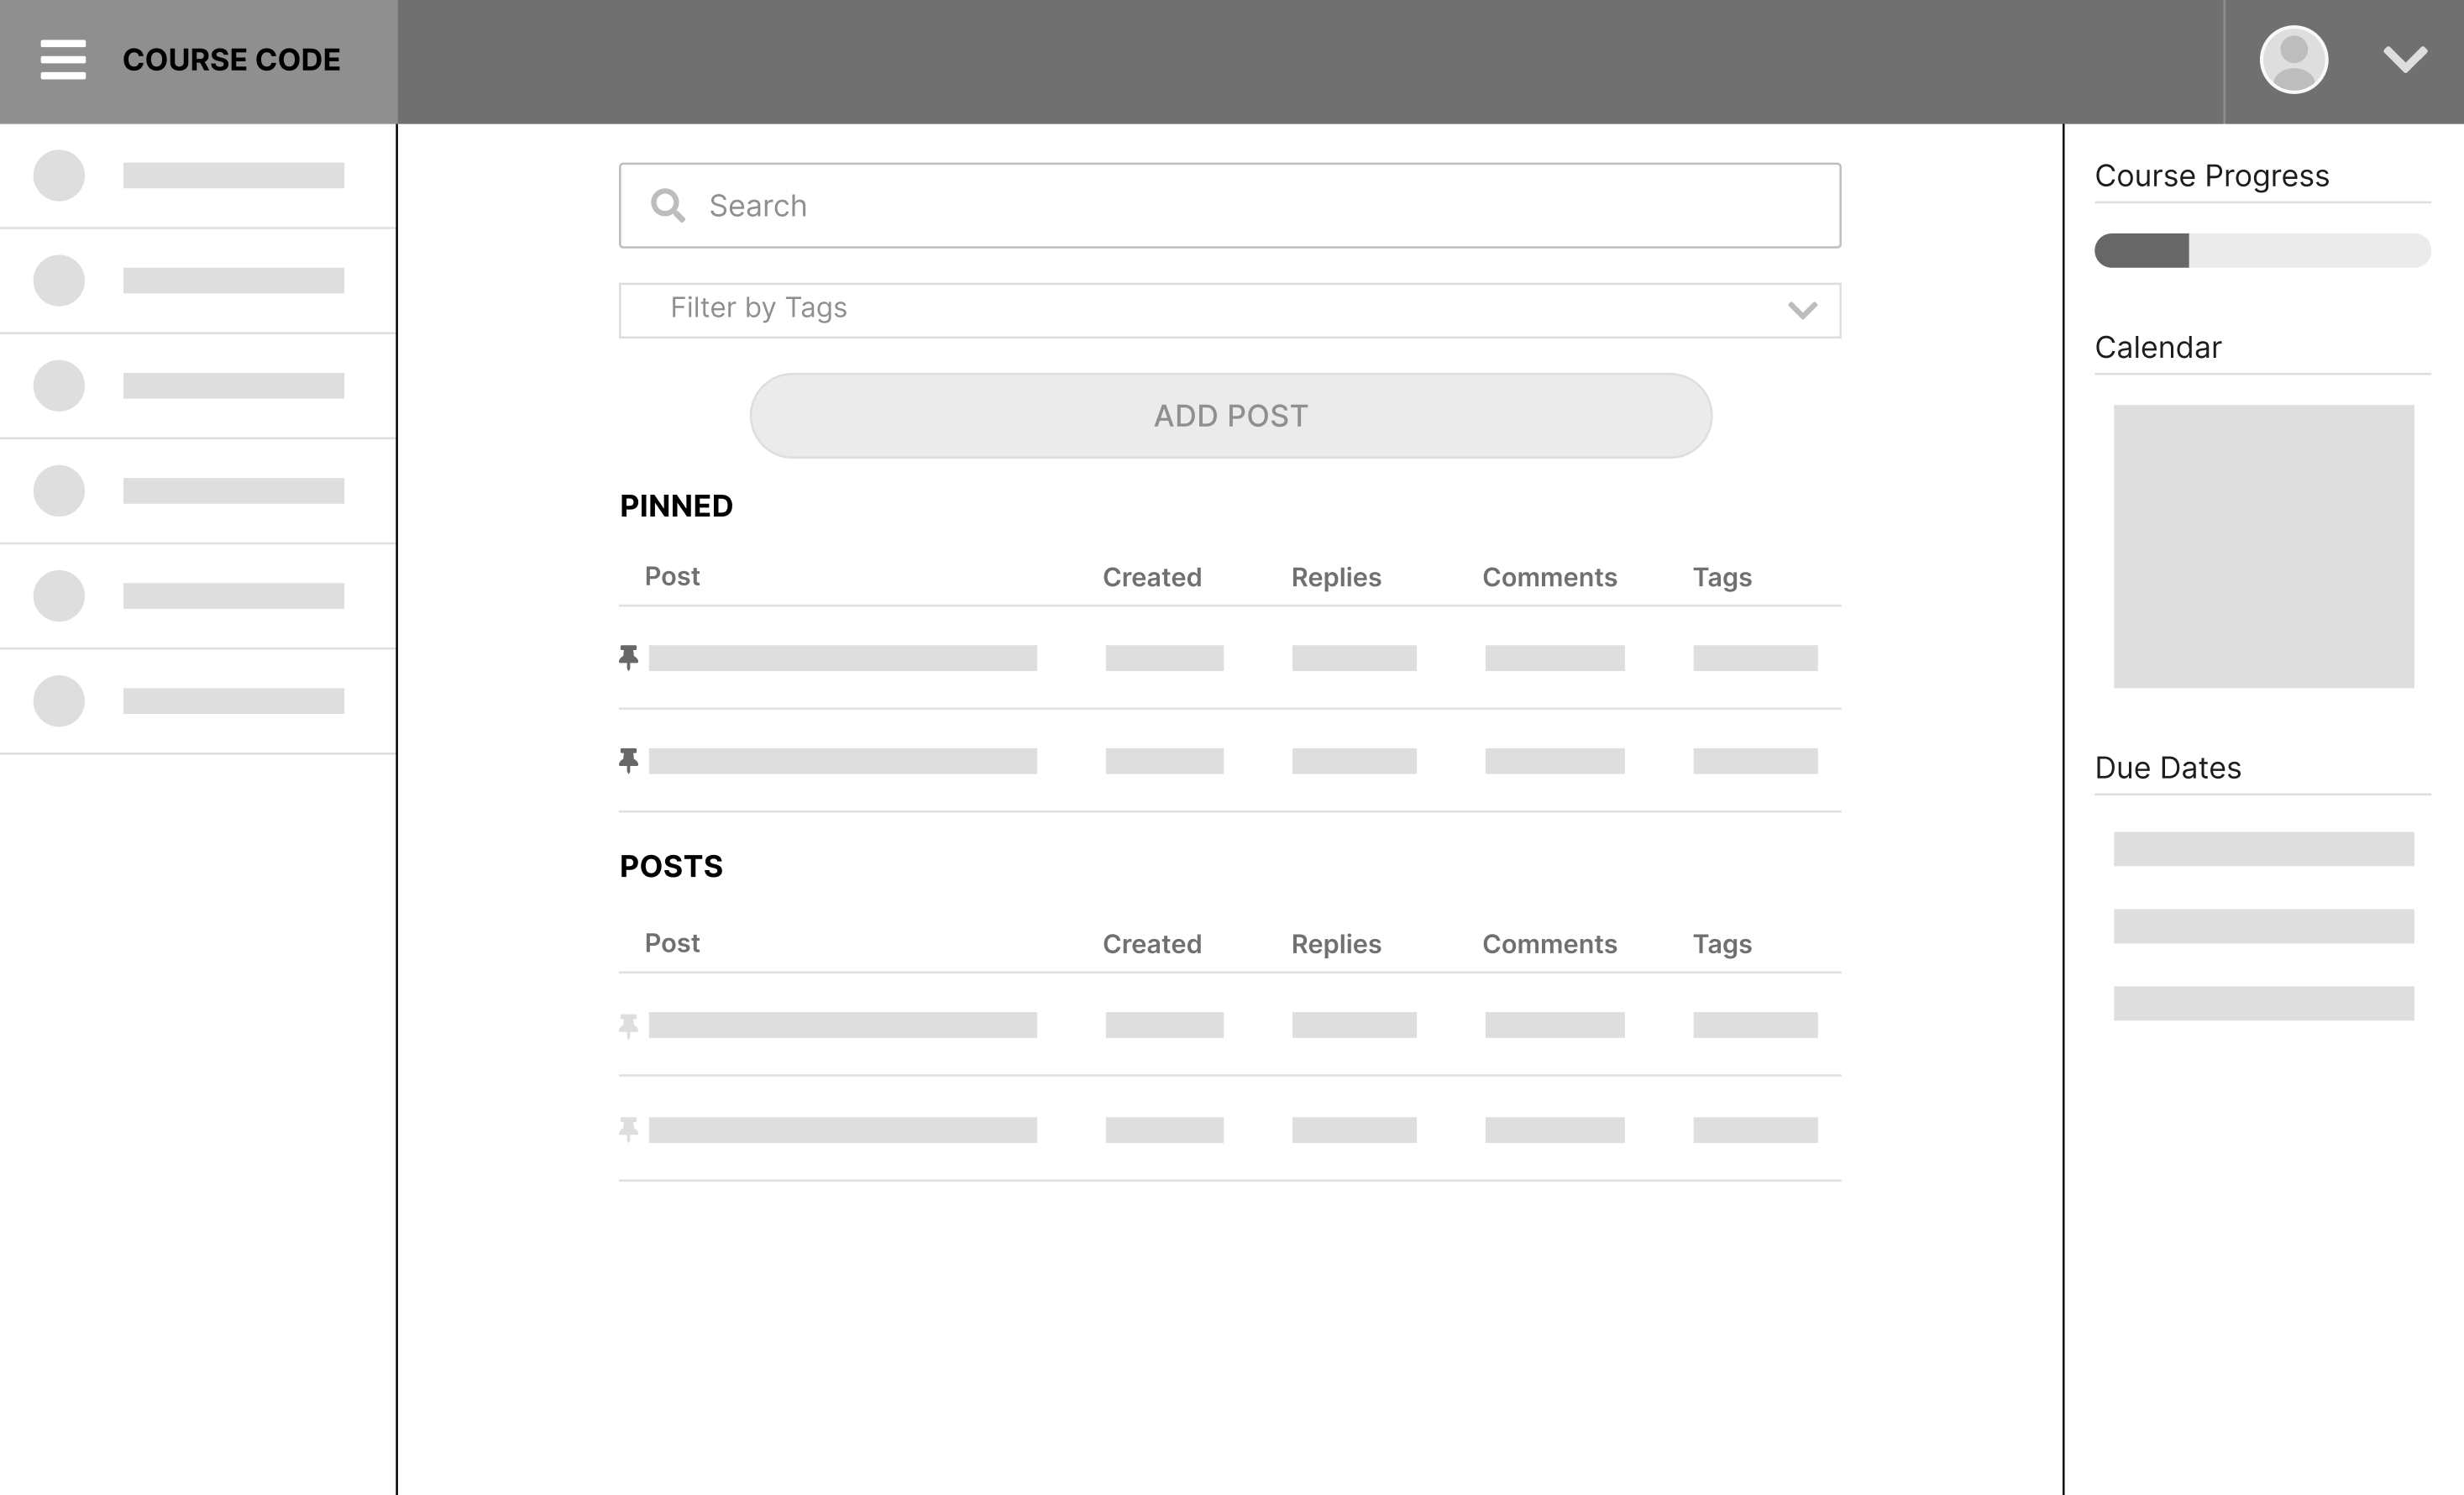
\includegraphics[scale=0.2]{forum-overview-page-admin.png}
    \centering
    \caption{Forum overview page for an admin}
\end{figure}

Admins have an additional button that allows them to pin and unpin posts.

\subsubsection{Post Page}

\begin{figure}[h!]
    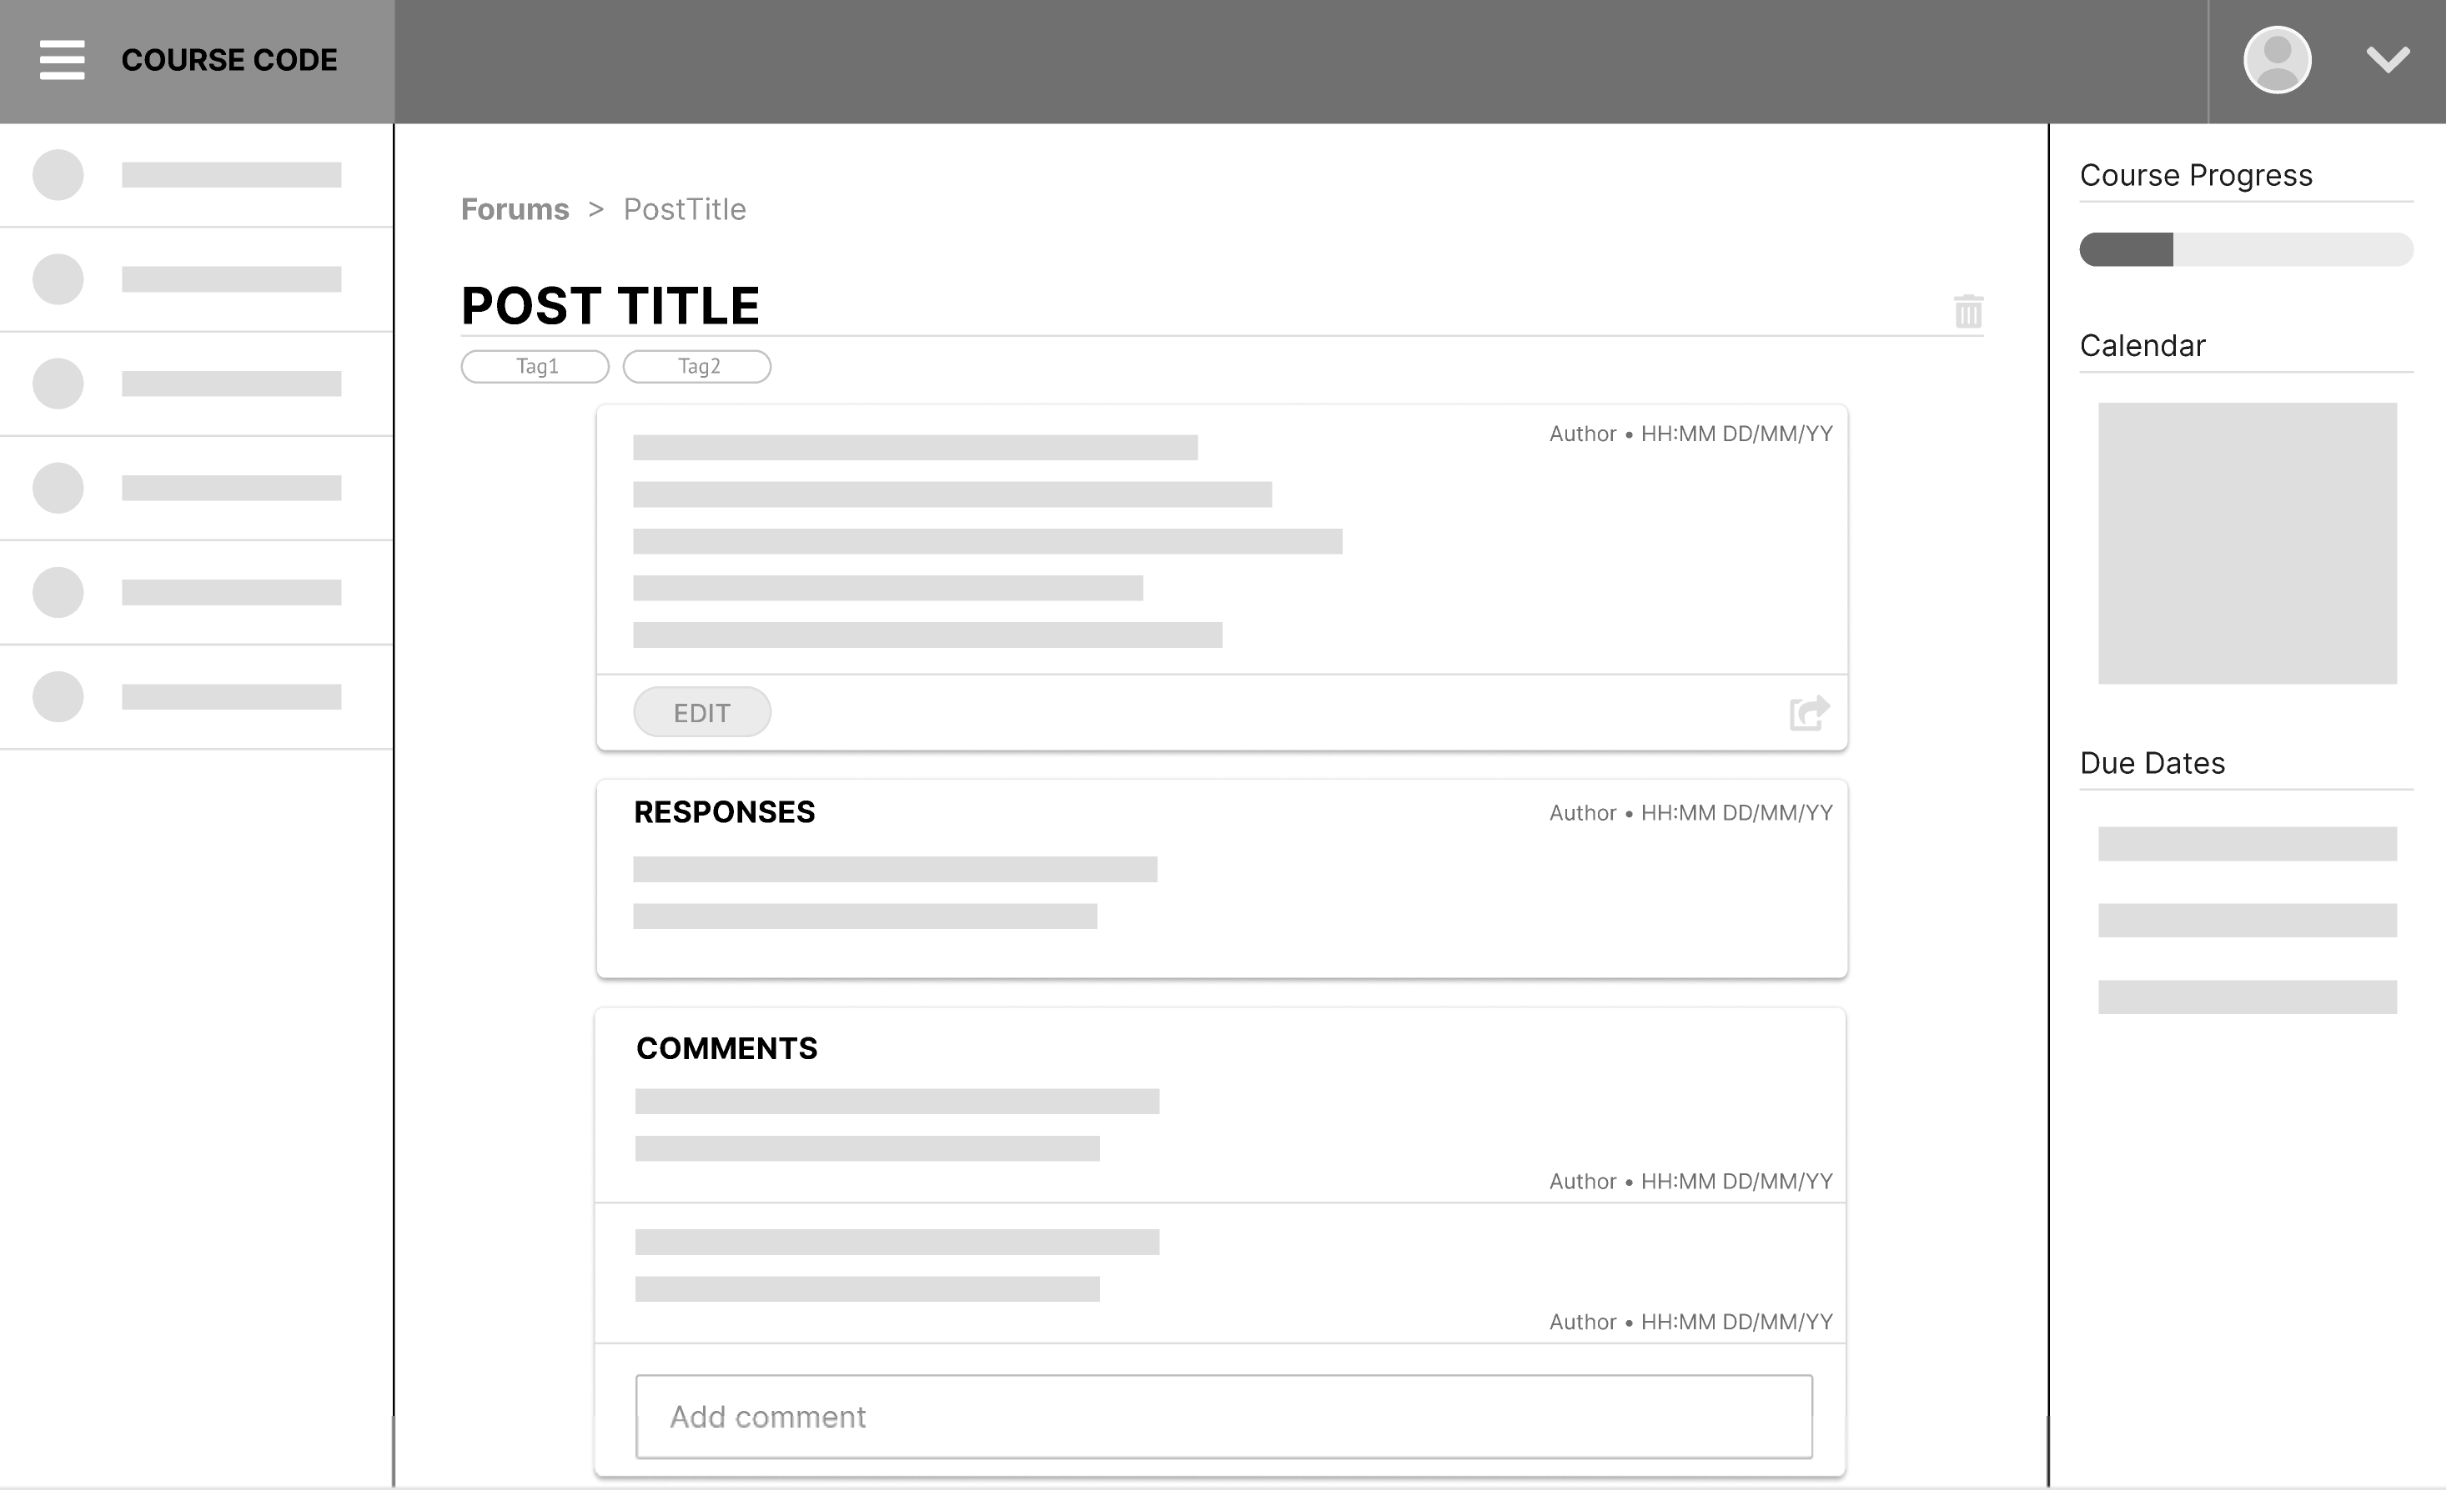
\includegraphics[scale=0.2]{forum-post-page-answered-student.png}
    \centering
    \caption{Forum post page for a student}
\end{figure}

Each forum post has its own post page which contains the post details, responses and comments.
Students are able to edit their posts from the post page if required.
They can easily view the instructor's response, if any, in the responses section.
The comments section allows the author to view and leave any additional comments.
It also gives other students a place to write a response or ask questions based on that forum post.

\begin{figure}[h!]
    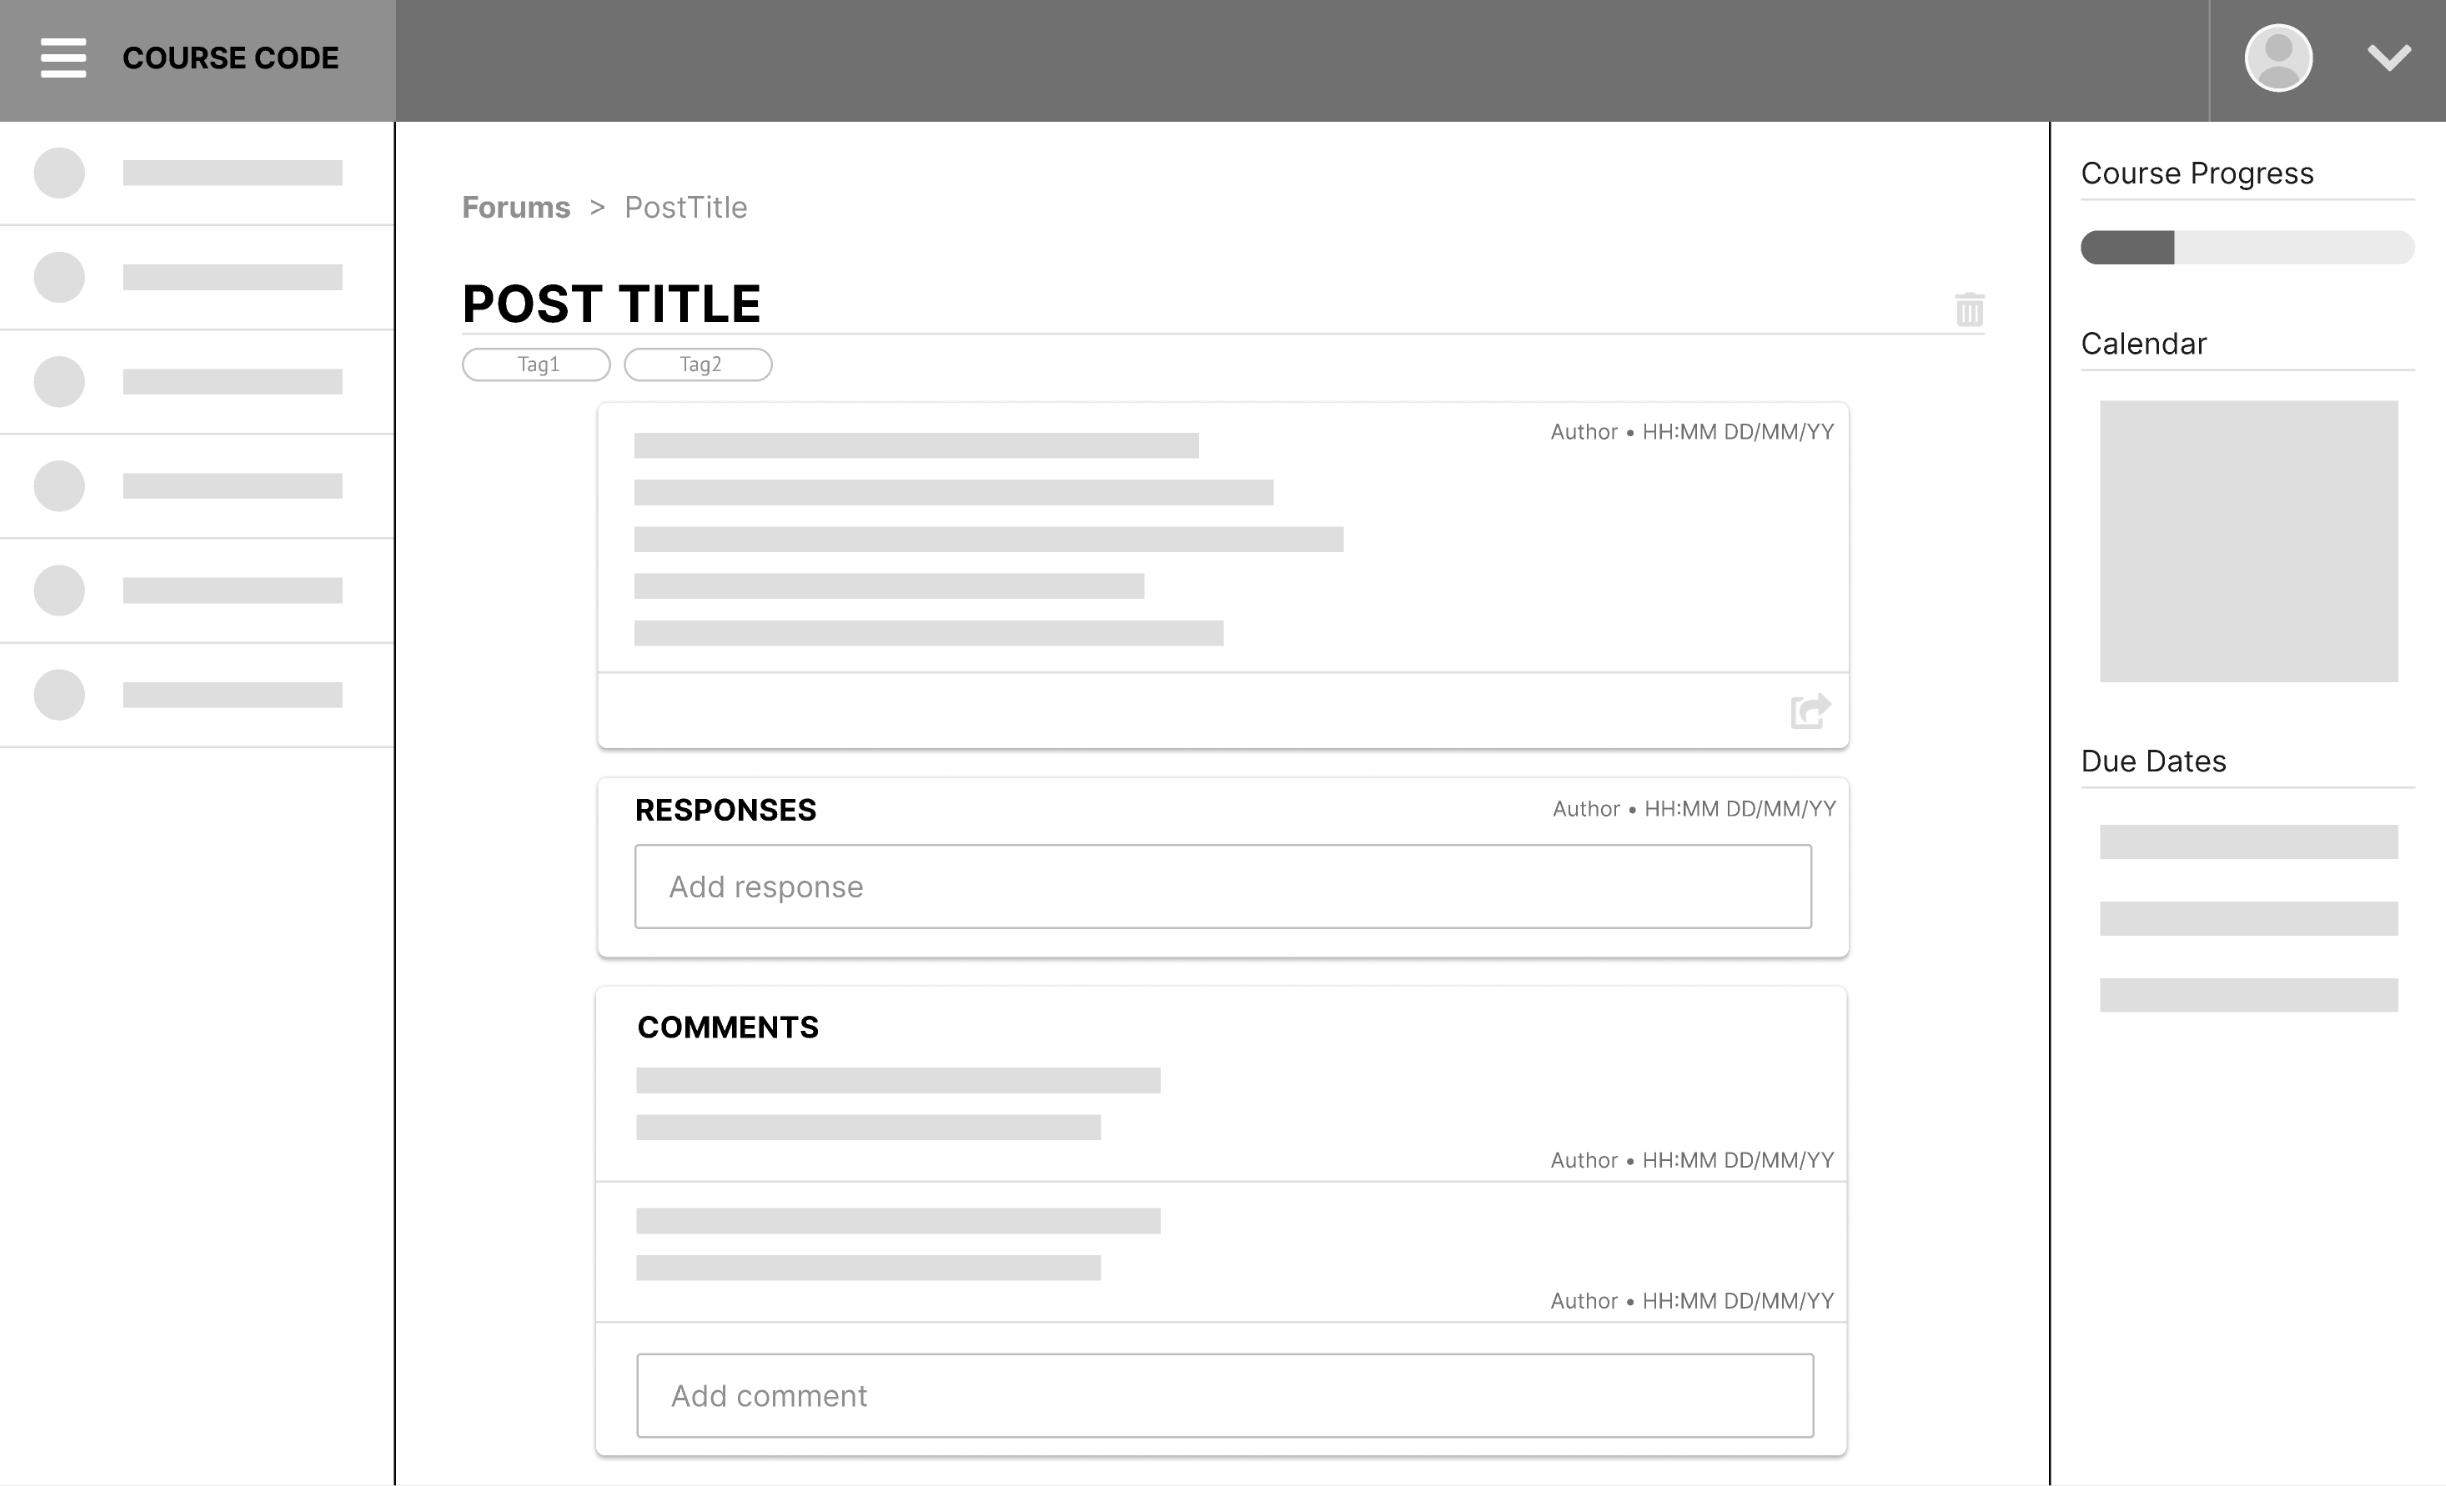
\includegraphics[scale=0.2]{forum-post-page-unanswered-admin.png}
    \centering
    \caption{Forum post page for an admin}
\end{figure}

If a forum post is unanswered, an admin is able to leave a response.
The current idea is to restrict this so that only admins can write responses to ensure that all responses are verified.
It also ensures that forum posts aren't left unanswered if a student accidentally leaves a follow-up question in the responses area, instead of the comments section.
This method of implementation may be reassessed if time allows.

\subsection{Requirements}
The following features are prioritised using the MoSCoW method which assists in identifying the order in which to implement the requirements.
It contains the following categories

\begin{itemize}
    \item \textbf{Must have} - vital features that are critical to the basic functionality of a project
    \item \textbf{Should have} - important features that aren't critical but add to the basic functionality of a project
    \item \textbf{Could have} - desired features that aren't necessary to the overall project but can provide a better user experience
    \item \textbf{Won't have} - low-priority features that likely won't be able to be completed in the given time-frame
\end{itemize}

\subsubsection{Functional Requirements}
\begin{enumerate}
    \item Users can view a list of forum posts (Must have)
    \item Users can make posts to the forum (Must have)
    \item Users can reply to forum posts (Must have)
    \item Users can embed images and links in their posts (Should have)
    \item Users can share forum posts (Should have)
    \item Users can categorise forum posts (Should have)
    \item Users can search forum posts (Should have)
    \item Users can clearly see which posts have been read and actioned (Could have)
    \item Admins can pin important forum posts (Should have)
    \item Admins can link/embed materials to forum posts (Could have)
    \item Admins can curate forum questions into collections (Won't have)
\end{enumerate}

\subsection{System Architecture}
Below is the recommended technology stack for implementing this forum system.
This stack has been chosen due to ease of use and past experience in developing with these technologies.

\subsubsection{Frontend}
In order to easily achieve the desired user interface, the following technology is recommended

\begin{enumerate}
    \item \textbf{React} - open-source frontend Javascript library
    \item \textbf{Material-UI} - React UI framework for quickly building components
    \item \textbf{CSS} - style sheet language for styling frontend components
\end{enumerate}

\subsubsection{Backend}
To handle the backend tasks, including storing and retrieving data, the following technology is recommended

\begin{enumerate}
    \item \textbf{Node.js} - open-source backend Javascript runtime environment
    \item \textbf{PostgreSQL} - open-source database management system
\end{enumerate}
